%
\documentclass[conference]{IEEEtran}
\usepackage{times}

% numbers option provides compact numerical references in the text. 
\usepackage[numbers]{natbib}
\usepackage{multicol}
\usepackage[bookmarks=true]{hyperref}
\usepackage{color}
\usepackage{graphicx}

%% Tarik's Shortcuts
% For marking TODOs in an obvious way
\newcommand{\TODO}[1]{ {\bf \textcolor{red}{TODO:} #1 }}

\begin{document}

% paper title
\title{Computer-aided design of complex configurations and behaviors for modular robots}

% You will get a Paper-ID when submitting a pdf file to the conference system
\author{Author Names Omitted for Anonymous Review. Paper-ID [add your ID here]}

\maketitle

\begin{abstract}
In this paper, we present a scalable software framework for the design of modular robot configurations and behaviors. Designs are constructed hierarchically by composing elements from a library, allowing users to easily create complex designs.  Likewise, complex behaviors are constructed by composing controllers from a library in a nested series/parallel structure. The system is integrated with a full dynamic simulator, and provides tools to identify common problems with behaviors, specifically self-collision and loss of quasi-static stability.

\end{abstract}

\section{Introduction}
\TODO{ Tarik writes} \\

Modular reconfigurable robot systems have been studied extensively for several decades \TODO{citations}.  These systems distinguish themselves in their ability to transform into different shapes to address a wide variety of tasks.

This additional flexibility places an additional burden on the user, because solving problems with modular robots involves not only designing  (software),
but also the best physical form for the task at hand. We argue that if this
complexity is not appropriately managed, it can make the system
impractical. �If the user is free to create any new design �he/she pleases to
solve a new task, but must program the design from scratch every time, creating
new designs will be a huge amount of effort, and the advantage of flexible modular
hardware will be defeated.

Software modularity is a well-established practice for developing large
maintainable systems and avoiding duplication of effort. �In robotics, software
behaviors are inextricably linked to the hardware they control, resulting in
additional challenges to modularity. �Significant progress has been made in
sharing robotics software between researchers
�and hardware platforms, most notably
�ROS which provides IPC and standard libraries for common robot tasks. 

The challenges of software design are different in modular robotics than
in typical robotics, because the hardware itself is modular. Porting software
from one robot platform to a completely different robot platform takes a
considerable amount of time, and needs to be facilitated by a large framework
such as ROS, in which fundamental software libraries are almost totally decoupled from
specific hardware. �In modular robotics, the emphasis needs to be on speed of
design, because the major advantage of a modular robot system is that new
designs can be made for each task. �We need to  very quickly develop simple kinematic
behaviors (take a step with a leg) with new morphologies that share some of the
structure of old morphologies.

Our solution to this problem is to let the modularity of our hardware drive the
modularity of our software. �We create new modular robot designs by combining existing sub-designs,
for example combining four leg designs with a body to create a walking robot.
�We provide a GUI tool that allows users to do this easily. �Designs have
associated libraries of software behaviors, so that when new designs �are created
by composing existing sub-designs, �new behaviors for that design can be quickly
and easily created by composing the behaviors associate with its component
sub-designs. �We introduce new scripting language with a series-parallel
execution structure that allows old behaviors to be easily and clearly combined
into new behaviors.

Since combining old things in new ways can lead to unexpected problems, we also
need to verify that our new designs and behaviors perform the way we expect them
to. �This is done in a dynamic simulation in Gazebo, and through
verification tools that detect common problems.


\section{Contribution and Paper Structure}

The primary contribution of this paper is a software system that allows modular
robot configurations and behaviors to be built hierarchically, and a simulation
environment that helps the user verify intended behavior.  Together, these tools
help manage the complexity of a modular robot system, significantly reducing the
time and effort required to accomplish tasks with modular robots.

The software we developed is open-source and freely available at [Link].  Our
code is built for SMORES,  a modular robot developed at the University of
Pennsylvania (see sec \ref{SMORES}), but could easily be adapted for use with
other modular robot systems.

The remainder of this paper provides a comprehensive description of the
structure and algorithmic components of our software system.  In Section \ref{sec:related-work},
we discuss relevant background material.
In Section \ref{sec:preliminaries} we introduce terminology and  concepts used elsewhere in the
paper. 
In Section \ref{sec:Approach_and_Algorithm}, we describe the algorithmic basis
for the three major components of our framework - design composition, behavior
composition, and behavior verification.  In Section
\ref{sec:Implementation-and-experiments}, we discuss the open-source software
tools used to implement our system, and provide examples demonstrating a user�s
workflow when using this system.  We demonstrate that our framework saves the
user time and effort, and allows him or her to easily develop complex and
capable designs.


\section{Related Work}
\label{sec:related-work}
\TODO{This is a work in progress.}
\begin{itemize}
\item Our effort is similar to what PPR/ROSLab is doing, but is specific to modular
robots. The design flow of our system is intended to be \textbf{faster} than that of
ppr, because our robots are modular. We only worry about connectivity,
not things like what motor to use.
\item The difficulty of programming new modular robot designs has been acknowledged
in the literature.  Quote from ``Modular Reconfigurable Robots, An Approach to Urban
Search and Rescue": `...the cost of programming systems is often more than the cost of hardware, thus reducing
the value of the flexible nature of hardware. \textbf{The extreme versatility of
n-modular systems requires a new paradigm in programming}
\item I have not seen any modular robotics papers that specifically address the difficulty
of (re)programming flexible hardware.
\item Many people focus on fully autonomous control and configuration selection algorithms.
\item Fully autonomous algorithms do not yet perform well enough to do useful things
with modular robots.  Therefore, we need a way for human beings to quickly and easily
create complex designs and behaviors. This paper presents a way to do that.



 \end{itemize}


\section{Preliminaries}
\label{sec:preliminaries}

\subsection{SMORES robot}
We have developed our system for the SMORES modular robot, developed at the
University of Pennsylvania \cite{Davey2012}. Each SMORES modules has four DoF
(DoF) - three continuously rotating faces we call {\em turntables} and one
central hinge with a $180^o$ range of motion (Figure~\ref{fig:SmoresRobot}). The
DoF marked 1, 2, and 4 have rotational axes that are parallel and coincident.
SMORES modules may connect to one another via magnets on each of their four
faces, and are capable of  self-reconfiguration.

Note that while we demonstrate our software with SMORES, it is not limited to the SMORES robot - it could be applied to any modular robot which may be simulated using Gazebo.


\begin{figure}[tb]
    \begin{center}
        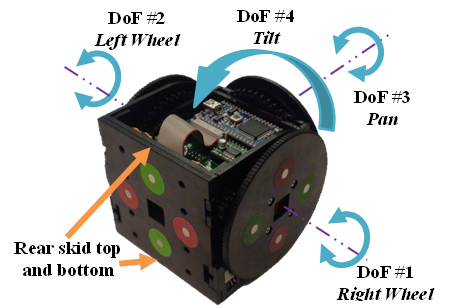
\includegraphics[width=\columnwidth]{images/smores_robot.png}
    \end{center}
    \caption{SMORES robot}
    \label{fig:SmoresRobot}
\end{figure}

\subsection{Concepts and terms}
A modular robot \textit{configuration} is a contiguous set of connected modules.  A configuration is defined by its connective structure, represented by a topology graph. \TODO{Define the graph}.

A \textit{behavior} for a modular robot is a programmed sequence of movements intended to produce a desired effect (such as walking). In this work, we represent open-loop kinematic behaviors using a \textit{gait table} data structure, which contain a time series of joint-angles for a specific configuration \cite{yim1994locomotion}.  In this paper, we consider only behaviors that can be represented using gait tables. \TODO{This is the typical definition of gait tables.  Ours are actually more complicated.  We need to come up with a precise, concise definition for them.}

A \textit{controller} is a position and velocity servo for one DoF of a modular robot.  A controller takes as input a desired position or angular velocity, and drives the error between the desired and actual state of the DoF it controls to zero over time.

When writing a behavior, it is possible to mistakenly command one controller to simultaneously hold more than one desired position; this is known as a \textit{controller conflict}.  Behaviors with controller conflicts are impossible to execute.

During execution of a behavior, a \textit{self-collision} can occur when two different parts of configuration are commanded to occupy the same location in space.  Self-collisions can damage the robot, and are usually unwanted.

In many cases, it is desirable to maintain \textit{quasi-static stability} during execution of a behavior \TODO{define}.

\section{Approach and Algorithm}
\TODO{Tarik and Jim write (see subsections)}
\paragraph{Configuration composition}
Define the composition of a set of configurations to a single configuration.

\subsection{Configuration Composition}
\TODO{Jim writes}
\paragraph{Input}
A set of configurations. A topology graph representing the connectivity among those configurations. A base module (for position transformation).
\paragraph{Output}
A composed configuration if it is safe.
\paragraph{Procedure}
\begin{itemize}
\item Start from the configurations that connects to the configuration with base module, transform their positions based on the position of the base configuration and topology graph.
\item Check if there is any collisions among the modules and report such collision.
\item \textbf{Check if the final configuration is stable. If not, find the plane that will make the configuration stable and transform the configuration.}
\item Show the expected behavior in simulator.
\end{itemize}

\paragraph{Controller composition}
Define the composition of a set of controllers to a single controller. Define the difference between a parallel composition and a series composition. Define the control composition graph.

\subsection{Controller Composition}
\TODO{Tarik and Jim write}
\paragraph{Input}
A configurations. A set of controllers. A control composition graph.
\paragraph{Output}
A composed controller if it is safe.
\paragraph{Procedure}
\begin{itemize}
\item Compose the set of controllers based on the given control composition graph. Explain how the parallel composition and series composition are handled.
\item\textbf{Check there is no controller conflict in the composition.}
\item Execute the composed controller in user defined incremental time interval. At each time step, update each module position and check collision.
\item \textbf{At each time step, check if the configuration will not have any unexpected behavior.}
\end{itemize}

\subsection{Complexity}
Discuss the complexity of the algorithm with respect to the number of modules and size of gait tables.

\section{Example and Experiment}
\TODO{Jim writes}\\
With simulation in Gazebo:
\begin{itemize}
\item Show a configuration composed from a set of basic configurations.
\item Show a composed controller that results in a collision in the configuration.
\item Show an updated controller that resolves the collision
\item Show a composed controller that results in an unexpected behavior.
\item Show an updated controller that eliminates the unexpected behavior.
\end{itemize}

\section{Conclusions}
We worked hard, and had fun.

\section{Future}
\begin{itemize}
\item How to represent different attribute/ability of the configurations
\end{itemize}




%% Use plainnat to work nicely with natbib. 

\bibliographystyle{plainnat}
\bibliography{references}

\end{document}




